\chapter{Introduction}

Annotating the content of unconstrained photos is a challenging problem. The primary complexity of photo annotation problems lie in their large search spaces and the diversity of feature-based representations of semantically similar images. Contextual information about a photo provides knowledge to prune this large search space, and simplify the task of feature-based classification techniques. The main intuition behind this work is that photos capture the state of the real world, and if we can reconstruct the various real-world entities and their relations at the time of photo-capture, this real-world context can prune the candidate search space. Ideally, the reduced search space will be orders of magnitude smaller, and will contain all the correct tags. In this work, we consider the problem of annotating faces in photos, where the search space consists of all possible people who can appear in a photograph.

Recently, the following changes in the technology climate motivate us to view real world information as context. First, with mobile phones becoming the primary mode of photo taking, the nature of context has evolved from providing cues about tags, to describing the world around a photo taking moment when a person was clicking the camera. Second, with the ever increasing amount of personal, social and public information, it is becoming harder to specify which subset of these would constitute the most interesting context for a given picture. Thus, it is not clear what source will provide context, and how do we combine them to form models of the real world which will allow photo annotation algorithms to reason what tags to assign various regions in a given photo. Finally, a large number of photos to be tagged today are \textit{personal} in nature. Tagging them is very different from tagging photos in datasets like LFW \cite{huang2008labeled} or Pascal-VOC \cite{everingham2010pascal}. Photos are created alongside other media (tweets, calendar entries, webpages), and a tagging system must take advantage of their inter-relationships.

% people are taking more photos, and tagging them requires deeper insights into how they are generated. very similar to how evolution is barely noticable at small time scales, but becomes prominent at larger ones (here we observer opposite phenomenon).

The most relevant context for a photo is contained in the relationships between the various real-world entities at the \textit{time of photo capture}. Given the various data sources and sensors, each of which contain partial information about these entities, it is non-trivial to meaningfully combine this information to produce the context for a photo. In this dissertation, we construct computational representations of such dynamic real-world entities and their relationships from the partial information in various heterogeneous data sources. We refer to such a representation as the \textbf{Context Network} of the photo. The network describes real-world events occurring with the photo-capture event, the objects participating in them, and their semantic inter-relationships. Given such a network for a photo, we can reason which parts of the search space can be pruned, and which of the remaining candidates are most likely present in the photo. 

\begin{figure}[t]
\centering
\begin{minipage}[b]{0.45\linewidth}
  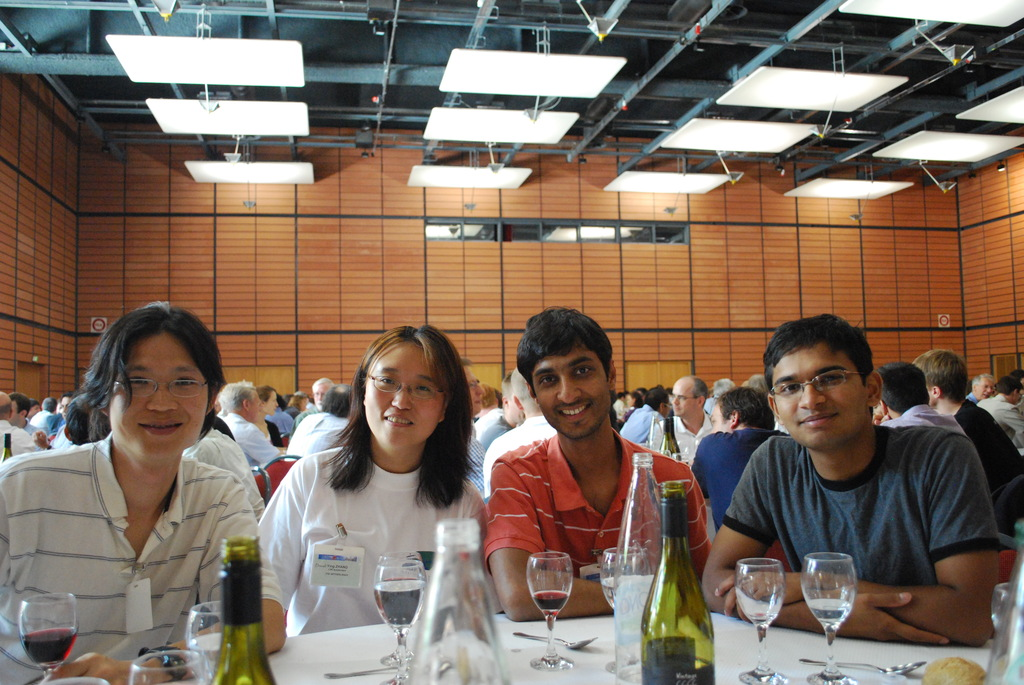
\includegraphics[width=\textwidth]{media/chapter1/vldb}
\end{minipage}
\begin{minipage}[b]{0.45\linewidth}
  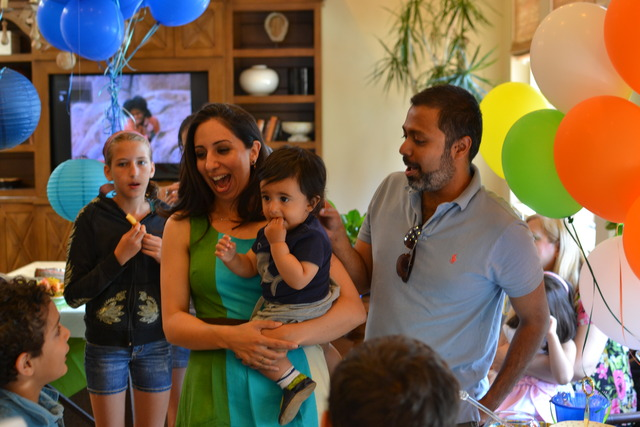
\includegraphics[width=\textwidth]{media/chapter1/nishkas}
\end{minipage}
\caption{Photos can be captured at a variety of different events.}
\label{fig:people}
\end{figure}

In this dissertation, we explore the symbiotic mutualistic relationship between contextual information and image features. Most often, context-aware multimedia problems use contextual information to simplify their respective challenges. But the opposite direction is undervalued and unexplored. A unified system where both contextual information can be discovered using images properties and image annotation can be achieved using contextual information forms the very novel foundation described in the following chapters. Such a \textit{systemic view} \cite{capra1997web} of context and image features where every component of a system assists the others, stands in contrast to \textit{pipeline systems} where every component provides appropriate inputs for the following components. By co-existing and supporting each other, the benefits of such a systems are very high, as shown below for the face tagging problem, specifically. 

\section{Importance of Context Discovery}

Annotation of multimedia artifacts such as images, audio and/or video clips \cite{galleguillos2010context, pang2011efficient, poppe2010survey, vinciarelli2009social, yang2010recognizing, zhao2003face, zeng2009survey} is a very active area of research. A technique to discover relevant context will play a large role in rendering such technologies more effective and allow them to operate in broader application domains.

Computer science is becoming largely utilized to address social \cite{sambasivan2010intermediated}, environmental \cite{ahrens2011data} and economic real-world problems \cite{chlistalla2011high}. Social network analysis, data-driven diagnosis in medical sciences, philanthropic engineering, monitoring public interests through real time communication networks, and situation-based advertising are some of the emerging applications of computer science. The common requirement for all of them is to construct real-world context networks. A technology to construct such unified representations from various data sources available today will play a key role in the scope and architecture of such systems.

For the purposes of this dissertation, we propose context discovery techniques in the light of photo annotation problems, but the technology and ideas are not tightly coupled with any singly media, and can be ported to assist in solving any problem which requires models of real world information.

\section{Context in Multimedia}

Context has been used to address many multimedia problems \cite{henter2012tag, li2012fusing, naaman2005identity, o2009context,stone2008autotagging}. For example, time and location information or social network information from Facebook to address the face recognition problem in personal photos. We refer to such a direct dependency between the search space and a data source as \textbf{static linking}. Although these systems are meritorious in their own right, they suffer from the following drawbacks: they are tightly coupled with a few data sources, the unavailability of any of which would reduce the efficiency of the system. They do not employ multiple sources synergistically, and therefore undervalue the \textbf{relations} between them. By realizing that these sources are interconnected in their own way, we are able to treat the entire source topology as a network, and traverse it to discover the relevant context.

\begin{figure}[t]
\centering
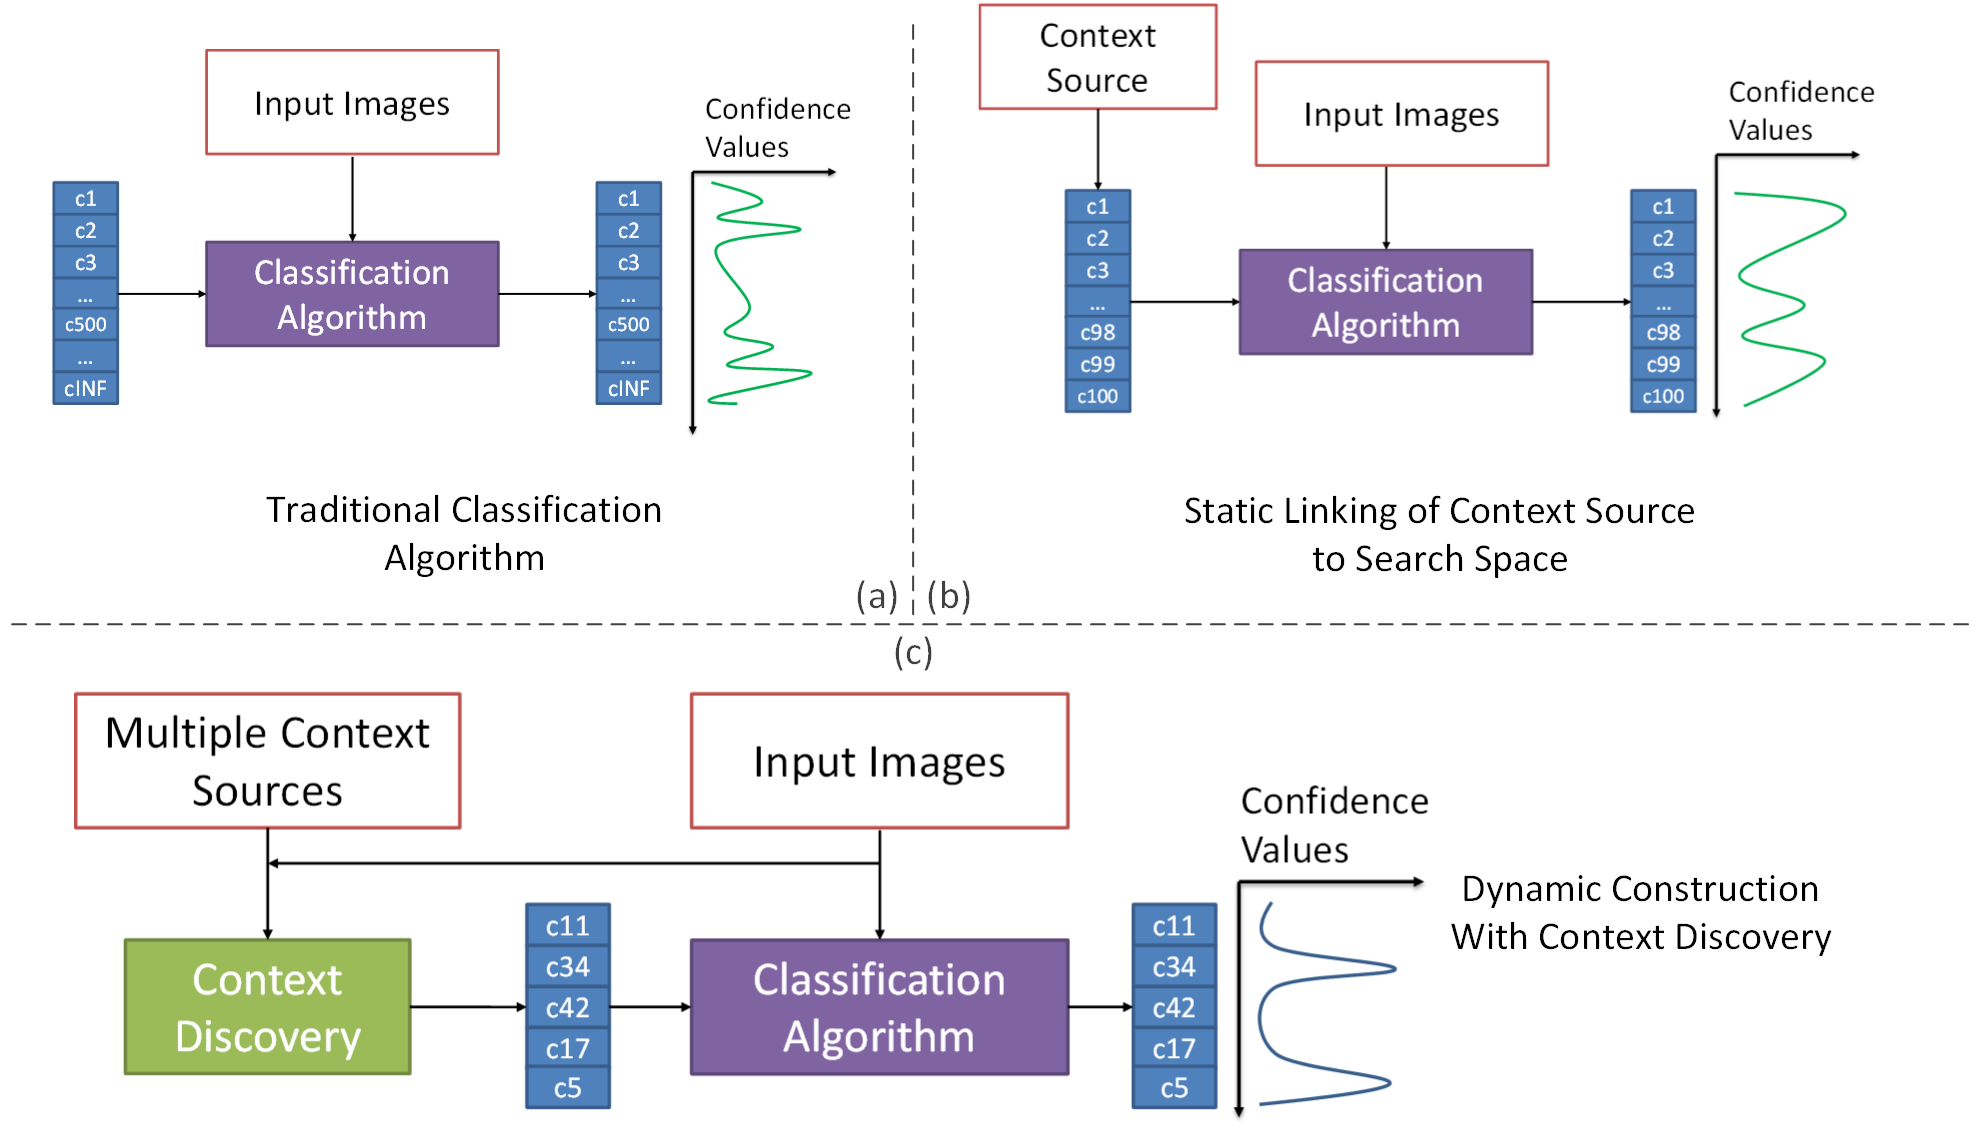
\includegraphics[width=0.85\textwidth]{media/with-without-cuenet-2.png}
\caption{The different approaches in search space construction for a multimedia annotation problem.}
\label{fig:with-without-cuenet-1}
\end{figure}

Figure \ref{fig:with-without-cuenet-1} shows three approaches to building photo annotation systems. Figure \ref{fig:with-without-cuenet-1}(a) is one of the earliest system setups where the search spaces were manually constructed, and the focus was mainly on constructing smarter features to correctly classify image regions \cite{belhumeur1997eigenfaces, turk1991eigenfaces}. Figure \ref{fig:with-without-cuenet-1}(b) shows systems such as \cite{stone2008autotagging} which use a single source, to populate their search space based on some attributes of the input problem (in this case, the identity of the user to query Facebook to discover relevant candidates). This restricts the search space but it assumes that all relevant tags will be supplied from the context source, which may turn out to be an expensive restriction. In contrast, our approach \textbf{dynamically links} context sources to the photo. We assume the availabilty of a large number of sources and sensors, but extract context from only a subset of them for a photo taken by a known user. Figure \ref{fig:with-without-cuenet-1}(c) shows how properties of input photo is used to reduce the search space. The properties are used to discover context, and prune the search space. This reduced space is considered by a face tagging algorithm to tag faces. Once the tagging is complete, any new information (new face tags) can be used to discover further context, and repeat the process till all the faces are tagged.

\section{Approach}
This primary \uline{contribution} of this dissertation is a \textbf{\textit{progressive discovery}} algorithm to ingest information from various real world data sources to construct context networks containing relevant information for pruning the search space of annotation problem. Examples of data sources include personal data sources such as personal calendar, mobile phone sensors (for example GPS which inform applications of the location of a person is present at any given point in time), personal emails, personal checkins on location services; social media web services to provide information about events and entities such as Facebook, Twitter; services which can be queried to find information about places such as Yelp; and finally public data sources such as Wikipedia, Upcoming, DBLP or websites on the world wide web which provide information about specific events (conferences or concerts).

In contrast to current static linking techniques, progressive discovery \textbf{dynamically links} context sources to the photo. It uses all available knowledge about a given problem (the input photo and related properties) to associate a subset of data from various sources as context. This allows us to decouple the technique of gathering context from the properties of the photo data. Because of this decoupling, there is no direct dependency on any specific set of sources, freeing the system developers to plug-and-play with various sources. With this decoupling, we are able to select different sources for different photos, and therefore discover only the relevant context for a given photo.



\section{Examples}
In this section, we present two examples of progressive discovery to demonstrate how different context is discovered for different photos. Figure \ref{fig:example-icmr-hidden} shows a photo of a person giving a presentation. Progressive discovery is done in three steps. First, the discovery algorithm proceeds to find the EXIF parameters and the camera device's owner with the photo. In our discussions we will use the term \texttt{photo-capture} event to signify the event in which a person clicks his/her camera and records a photograph. The event is assumed to contain spatio-temporal attributes which specify when and where the photo was taken. In the next step, these spatio-temporal attributes are used to discover \textit{what events, if any, is this object (the owner) participating in, at this time}? Only those data sources are searched which can provide results to such a query (for example, facebook's social network will not be searched, as it does provide temporal information about people). We obtain a response from a conference database saying that the owner was attending the ICMR conference at Dallas, Texas. Third, given this new conference event, the algorithm discovers what conference subevents (keynotes, talks or break sessions) were occurring at this time. Finally, it finds that Mor Naaman and John Smith were speaker and host respectively, for the keynote talk going on that time. Given the two candidates, the face tagging algorithm proceeds to identify Mor Naaman as the person in the photo, as shown in figure \ref{fig:example-icmr-show}.

\begin{figure}[ht]
\begin{minipage}[b]{0.45\linewidth}
\centering
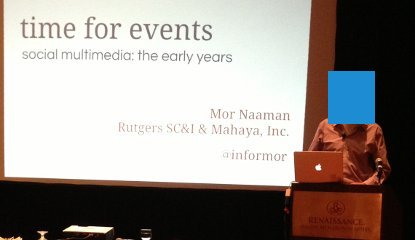
\includegraphics[width=\textwidth]{media/chapter1/icmr-keynote-2-hidden.jpg}
\caption{Who is in this photo?}
\label{fig:example-icmr-hidden}
\end{minipage}
\hspace{0.5cm}
\begin{minipage}[b]{0.45\linewidth}
\centering
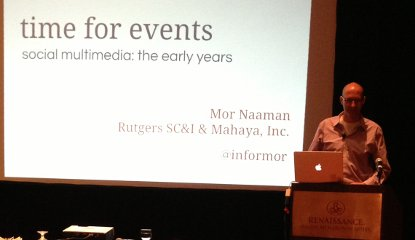
\includegraphics[width=\textwidth]{media/chapter1/icmr-keynote-2-show.jpg}
\caption{Mor Naaman at ICMR.}
\label{fig:example-icmr-show}
\end{minipage}
\end{figure}

Now, let us attempt to discover context for photo shown in figure \ref{fig:example-kasturi-hidden}. Context discovery initiates the same way as in the above example, but after searching for events related to the owner in data sources, finds nothing. It proceeds to rank all known contacts according to location, and given that this photo was taken to the owner's workplace ranks colleagues higher than friends. The top 20 (an arbitrary constant) ranked candidates are passed to the face tagging algorithm which finds Ramesh Jain in the photo. But not the person to his right in the photo. Since the \texttt{photo-capture-event} has an additional participant, Ramesh, his personal information (calendar or social network) can be queried to find events in which he was participating. The calendar returns the entry ``Kasturi". The algorithm uses this term to find all Ramesh's contacts to find all people with first or last name ``Kasturi'', and finds his long time friend and colleague ``Rangachar Kasturi''. The face tagging algorithm is invoked with one candidate. In this case, it is simply checking if Prof. Kasturi is present in the photo or not.

\begin{figure}[ht]
\begin{minipage}[b]{0.45\linewidth}
\centering
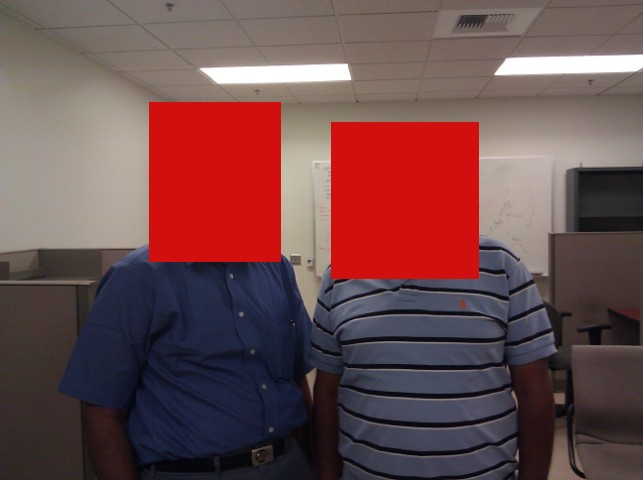
\includegraphics[width=\textwidth]{media/chapter1/kasturi-hidden.jpg}
\caption{Who is in this photo?}
\label{fig:example-kasturi-hidden}
\end{minipage}
\hspace{0.5cm}
\begin{minipage}[b]{0.45\linewidth}
\centering
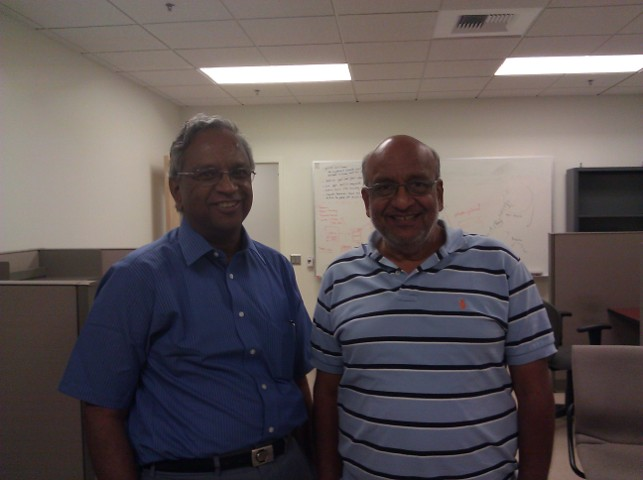
\includegraphics[width=\textwidth]{media/chapter1/kasturi-show.jpg}
\caption{Kasturi and Jain.}
\label{fig:example-kasturi-show}
\end{minipage}
\end{figure}

In this first run, the algorithm links only to a conference database, whereas in the second case, it used spatial information, personal calendar and contact information. For the first image, we did not link social networking or contact information to the image, and similarly, conference databases were not linked to the second image. This variation in linking to sources is an example of dynamic linking. In the later chapters, we will present techniques to represent and link context in a systematic manner.

\section{Overview}
This dissertation is organized into the following chapters. Chapter 2 provides an overview of context, how context has been used to address problems in various scientific disciplines and how we use context in our specific personal photo tagging application. Chapter 3 describes the related work in computer science, specifically the main ideas in photo annotation and tag propagation techniques, and presenting the techniques prevalent in context modeling and processing communities: how context is used to solve problems in different domains. Chapter 4 describes our context discovery framework, how it models various data sources, and how our progressive discovery algorithm constructs models for real world problems. We facilitate this discussion with an example real world application to tag faces of people in personal photos. Chapter 5 analyzes the algorithmic complexity of different parts of the system, and provides experiments to verify the competence and performance of the system. We also present experiments to confirm the efficacy of our approach in the light of the real world application. Chapter 6 presents a technique to use previously tagged photos and their context networks to rank candidates in context networks for new photos. Finally, chapter 7 describes the known issues of our approach and the future possibilities of using context discovery in various applications.